\graphicspath{{images_low_res/}}
\section{Approach}
\label{sec:approach}

\subsection{Develop an Initial Model}
\label{sec:initial_model}

Figure~\ref{fig:simple_model} shows a schematic of our initial
approach to consttucting a competition for nutrients and signalling
(CANS) model. Each culture at location, \(i\), is associated with
three variables: one observed variable, \(C_{i}\), the amount of cells
\(i\), and two hidden variables, \(N_{i}\) and \(S_{i}\), the amount
of nutrients, and signal. Cultures in QFA and SGA agars are arranged
in a square array, each culture having eight neighbours with which
they could conceivably interact directly. Initially, we will
model diffusion between only the four closest neighbours, indicated by the
darker blue circles in Figure~\ref{fig:simple_model}. Assuming a well
stirred mixture, we will describe nutrient dependent growth at each
location using mass action kinetics and the following reaction
equation:
\begin{equation}
  \label{eq:2}
  C + N \xrightarrow[]{r_{i}} 2C,\\
\end{equation}
where \(r_{i}\) is the rate constant of conversion at location \(i\).
As a first approach, assuming that the number of cells is continuous,
we will incorporate the effect of signal molecules on growth and the
diffusion of both signal molecules and nutrients using the following
ODEs (CANS model):
\begin{subequations}
  \label{eq:3}
  \begin{align}
    \frac{dC_{i}}{dt}& = r_{i}N_{i}C_{i} - \beta S_{i},\\
    \frac{dN_{i}}{dt}& = - r_{i}N_{i}C_{i} - k_{n}\sum_{j}(N_{i} - N_{j}),\\
    \frac{dS_{i}}{dt}& = \alpha C_{i} - k_{s}\sum_{j}(S_{i} - S_{j}),
  \end{align}
\end{subequations}
where, \(j\) indicates the closest neighbours, \(k_{n}\) and \(k_{s}\)
are nutrient and signal diffusion constants, \(\alpha\) is the rate of
secretion of signal, and \(\beta\) is a constant for the effect of
signal on culture population. ?do we assume no cell death\ detect dead
cells on the agar/ times are short? Alternative models of signalling
effect could be used, depending on the mechanism of signalling under
investigation (see background section); initially, we have chosen to
use the simplest modelling approach. Setting diffusion constants to
zero reduces \ref{eq:3} to the independence model. We may also study
the effects of signalling and competition for nutrients separately by
setting other parameters to zero. If necessary, diagonal neighbours
could be incorporated by adding or scaling diffusion constants. In
section~\ref{sec:dev-mod-further}, we discuss the possibility of using
finer-grain spatially-discretised or continuous models of diffusion
which would also achieve this.
% \begin{equation}
%   \label{eq:4}
%   \frac{dC_{i}}{dt}& = r_{i}N_{i}C_{i}(1 - \frac{S_{i}}{S_{crit}})
% \end{equation}

\begin{Figure}
  \centering
  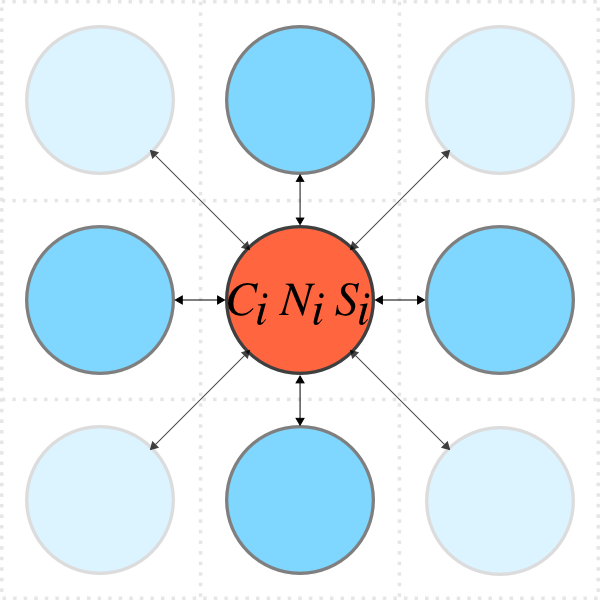
\includegraphics[width=\linewidth]{square_array}
  \captionof{figure}{Schematic of simple modelling approach.}
  \label{fig:simple_model}
\end{Figure}

Models will be written in SBML (ref), using SBML shorthand (ref), so
that they may eventually be published in the BioModels database (ref)
and available publicly. This will require conformation to the minimum
information standard MIRIAM (ref). (Simulation experiments should also
conform to MIASE (ref).) We will write code for the rest of the
project in Python as this has several advantages: it is used widely by
the scientific community, has libraries which will be of use to us,
and related tools such as Colonyzer \citet{Lawless2010} are already
written in Python. To interface SBML models with Python we will use
the libSBMLO library \citep{Bornstein2008}. ODEs will be solved using
odeint from the SciPy library \citep{SciPy}. We will use git as
version control and GitHub as a remote repository where packages will
eventually be released publicly.

It is anticipated that solving sets of ODEs for typically 384 cultures
in QFA and 1536 cultures in SGA will be take a long time. Therefore,
in the testing stage, we will simulate smaller sets of artificial data
from the ODE models and attempt to fit these. We will also incorporate
unittesting into the development to try to ensure that code will
still work when scaled up to larger arrays used in experiments.

When dealing with experimental data we must also consider how to treat
cultures around the edge of the agar. These have access to
proportionally more nutrients because there is a relatively large area
beyond them which is unoccupied by cultures. In photographic images,
these sites are also affected by reflections from plate walls which
cause errors in integrated optical density (IOD) measurements, a proxy
for cell density, which cannot be fully corrected for by Colonyzer
\citep{Lawless2010}. In experiments, an identical culture is grown in
edge locations and the results are discarded (see refs). We may choose
to adjust for the increased nutrient access and include edge cultures
in our model and analysis. This would introduce a systematic error for
sites close to the plate edges and is an argument for the use of
repeats and randomisation of location (see
\ref{sec:comp-exper-designs}). A simpler modelling approach is to
discard the first outer layer entirely from the model and the second
outer layer from the final results. However, this is undesirable as it
reduces the amount of information that is gathered from each plate and
may not account for the systematic error any better than the more
complicated approach, possibly allowing it to propagate further.

\subsection{Analyse Experimental Data}
\label{sec:analyse-data}

List of strains of known fitness??

We have access to unpublished QFA and SGA data for the model organism
\textit{S. Cerevisiae}. Some data (Figure~\ref{fig:gaps}), with vacant
gaps, is specifically designed for the study of
competition. ?presumable some with the same variants grown on the
plate?. We will analyse data from single plates to avoid having to
deal with batch variance which can be a major source of error (see
\citet{Baryshnikova2010}). We will at first fit our model to data
using least squares. The QFA R package (ref) contains functions for
fitting the independent logistic growth model and there is development
underway of a qfaBayes package (ref) which will carry out a Bayesian
inference of parameters of the same model. We plan to develop a method
for Bayesian inference using the CANS model which will account for our
prior knowledge/?belief? about parameters distributions (?any other
advantages?) (?and allow us to conduct model comparison?). In an
analysis of high-throughput QFA data from a genetic interaction study
by \citet{Addinall2011}, \citet{Heydari2016} use a Bayesian
hierarchical model which mirrors the exerimental structure (from the
time-point to population level) and simultaneously estimates growth
parameters and genetic interaction strength by sharing information
between levels. This approach accounts for differences in replicate
fitness variances between different mutant strains which cannot be
efficiently factored into statistical analyses
\citep{Heydari2016}. When looking at the most significant genetic
interactions, for the increased computational time that it takes (4
weeks vs 3 hours), this analysis does not offer a significant
advantage over an earlier statistical analysis carried out by
\citet{Addinall2011}. However, \citet{Heydari2016} do identify weakly
interacting genes for which there is no previous evidence, and a
hierarchical model which only modelled population dynamics took
significantly less time (1 week). As we are only studying single
plates and not going on to infer genetic interaction strength, there
will be fewer levels in our hierarchy, allowing for a faster
computational time, and the analysis may provide more significant
evidence in identifying competition effects than it does for genetic
interactions (?is this last bit true? ?should we discard this or
not?).

\begin{Figure}
  \centering
  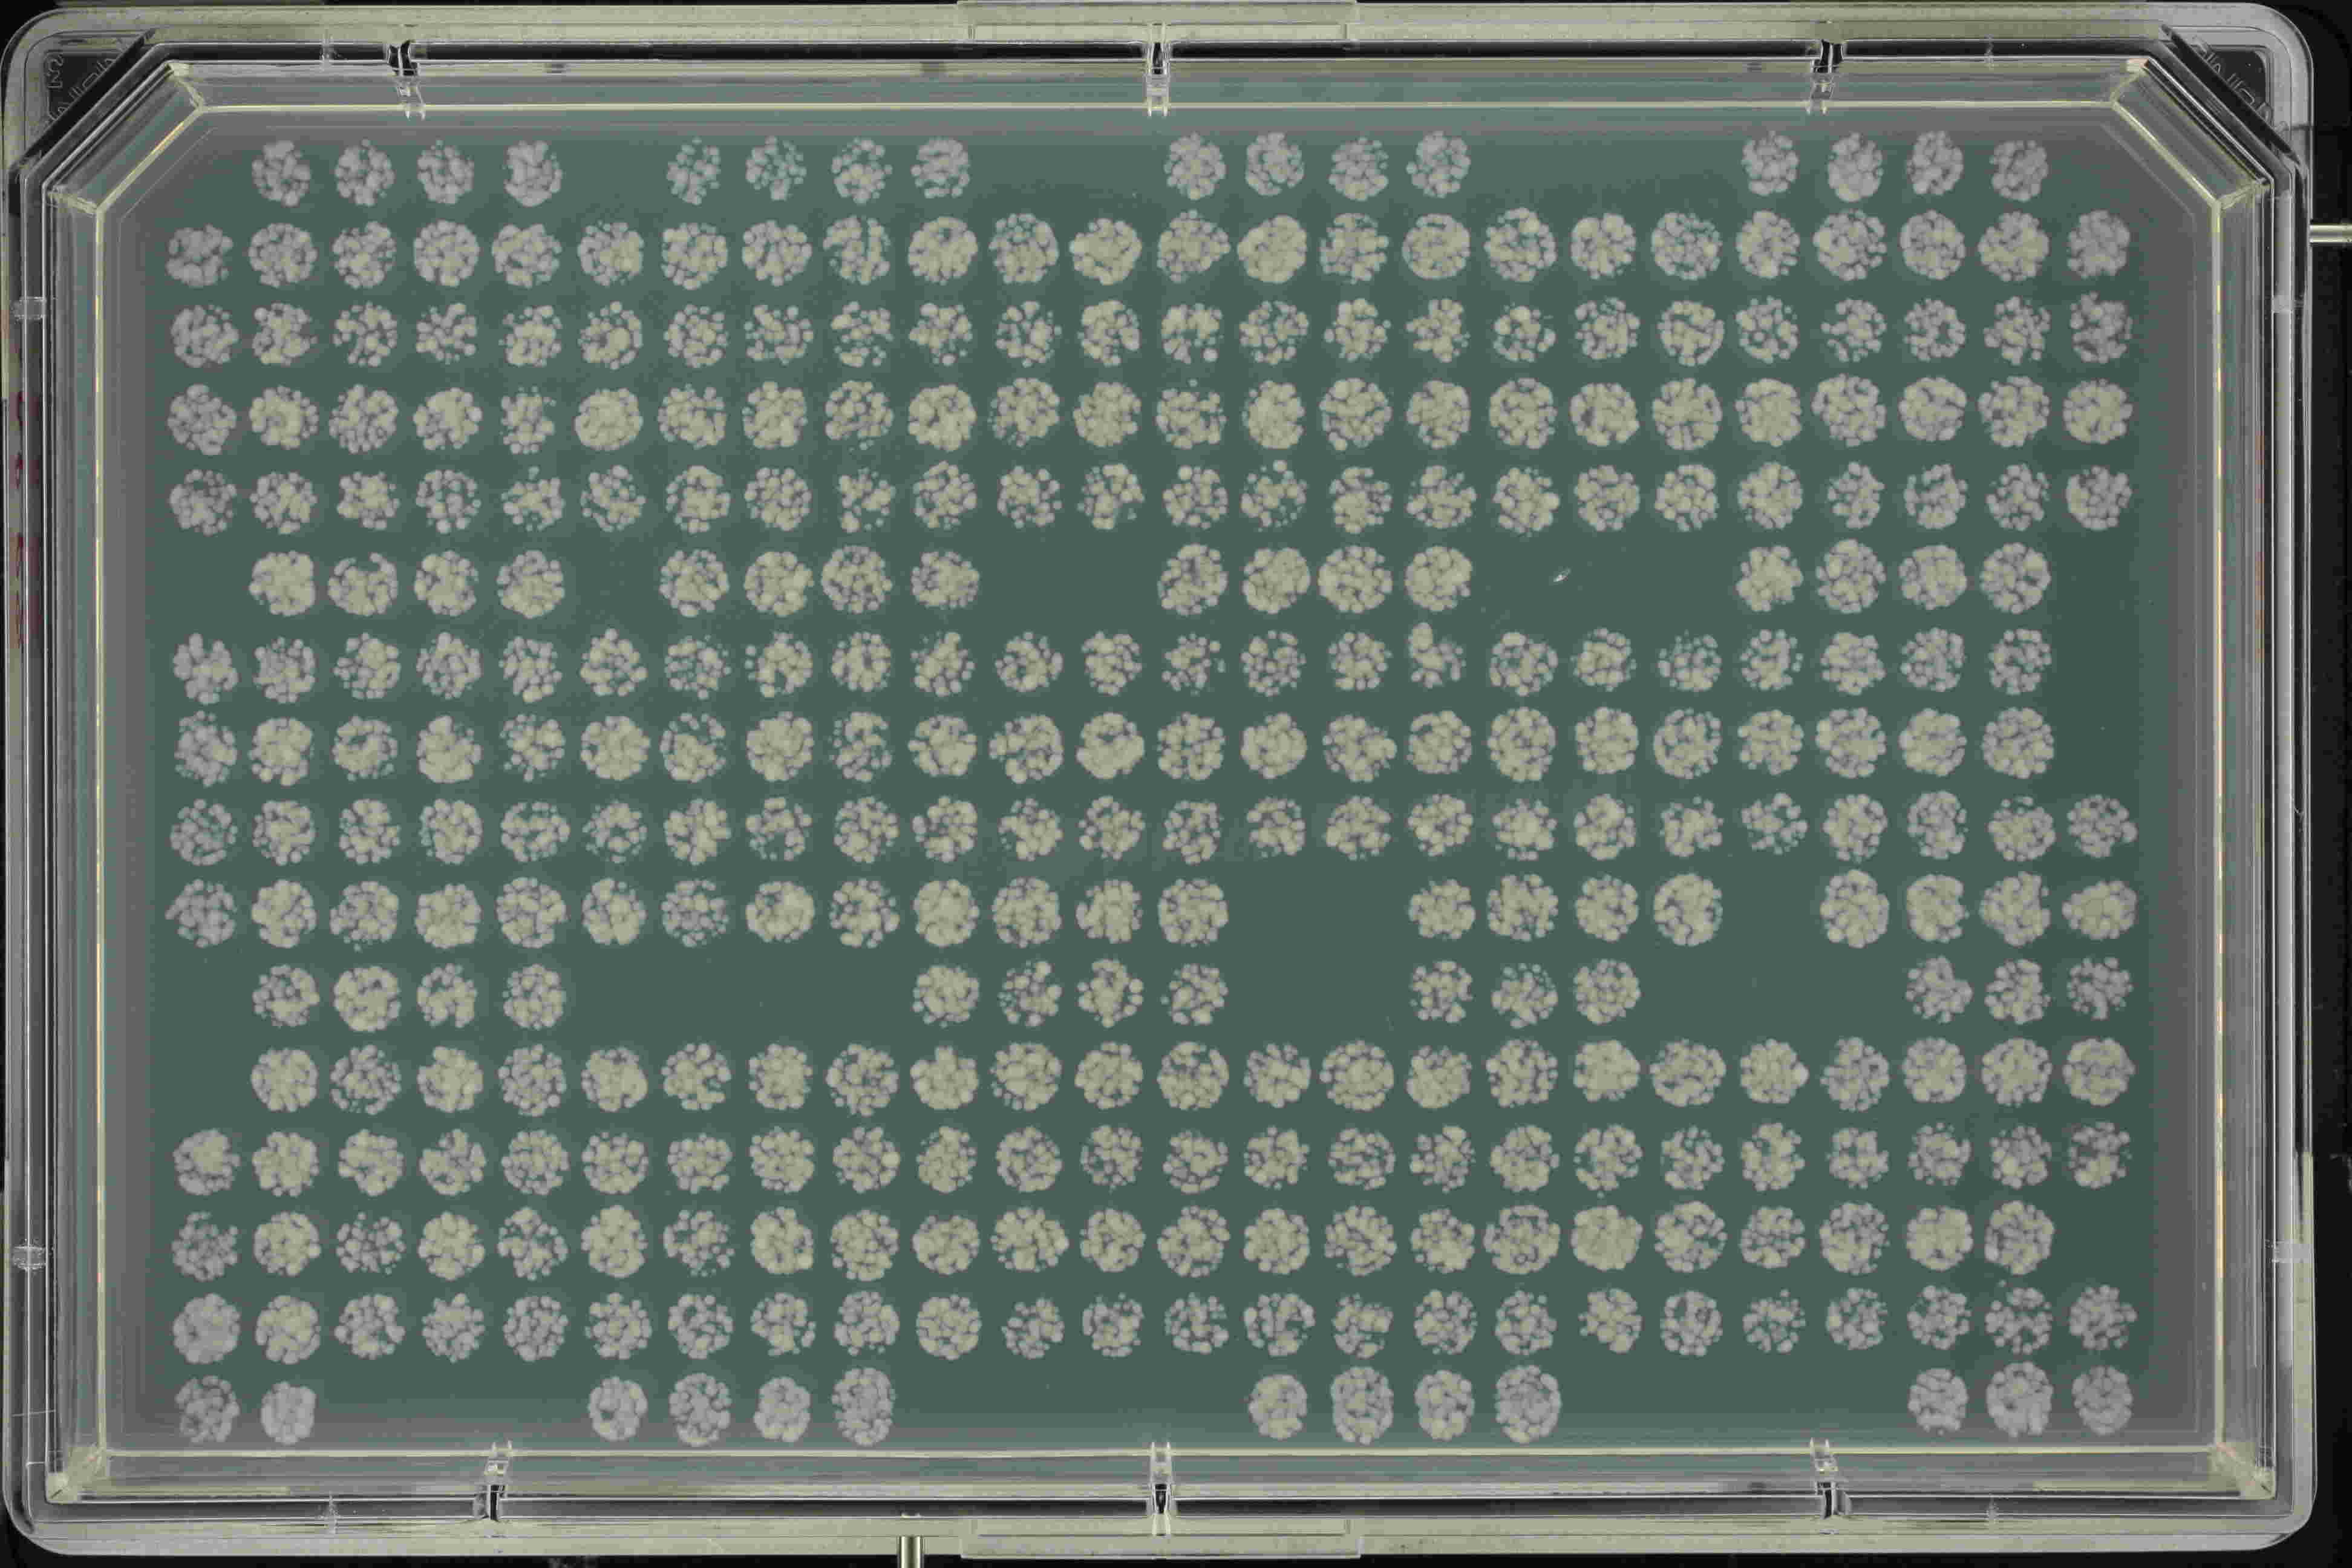
\includegraphics[width=\linewidth]{DLR00012647-2009-07-02_23-12-49}
  \captionof{figure}{An agar with locations left empty (``gaps'')
    designed to exhibit effects of competition and signalling.}
  \label{fig:gaps}
\end{Figure}

If we fail to discover competition or signalling effects by fitting
the CANS model, we may need to improve aspects of our modelling
approach (see section \ref{sec:dev-mod-further}), study different
data, or consider that the data is not subject to these effects. (The
latter conclusion would raise questions about other sources of
variance.) Otherwise, if we find evidence of a significant competition
and/or signalling effect, we have proved our main hypothesis and can
move on to comparing experimental designs (section
\ref{sec:comp-exper-designs}). In order to compare diffusion across
agar height we will need to develop a two-dimensional
spatially-discretised model of diffusion (section
\ref{sec:dev-mod-further}.

We will also determine the effect of competition on the different
measures of fitness discussed in section
\ref{sec:genetic-interaction}. In previous studies, which use fits of
the (independent) logistic growth model (refs), fitness estimates
based on carrying capacity \(Z\) might be more affected by competition
and signalling than those based on rate constant \(r\). This is
because gradients in nutrient and signal density will likely be
greater towards the end of growth curves, after the exponential growth
phase, when cultures are larger and have grown for longer. To asses
this possibility, we initially attempt to model competition for
nutrients in terms of parameters of the logistic growth model using a
time dependent carrying capacity,
\begin{equation}
  \label{eq:5}
  Z_{i}(t) = Z_{0,i}\left(\frac{N_{0,i} + \Delta N_{i}(t)}{N_{0,i}}\right),
\end{equation}
where \(Z_{0}\) is the carrying capacity under the assumption of
independence, and is modified by the ratio of net nutrients available
at time \(t\) to the initial amount of nutrients available under the
assumption of independence \(N_{0}\). In this model, the form of rate
constants \(r_{i}\) in \ref{eq:1} is unaltered. Before fitting this
model to data, we would first need to find \(\Delta N_{i}(t)\), the
integral of the second term in \ref{eq:3}b, by fitting a nutrient only
version of \ref{eq:3}. It would take further work to find exact
relationships between parameters of \ref{eq:1} and \ref{eq:3} and to
include signalling in the model. ?Conor,
you said you might have done this previously?  ?Also, is what I have
suggested above sensible?

\subsection{Develop Model Further}
\label{sec:dev-mod-further}
If we find that our initial CANS model offers no improvement over the
independent model, or is in some other way inaccurate, we could
consider improving the model in several ways. For instance, we may
propose a different model of signalling effect and instead model
culture growth rate as,
\begin{equation}
  \label{eq:6}
  \frac{dC_{i}}{dt} = r_{i}N_{i}C_{i}\left(1 - \frac{S_{i}}{S_{crit}}\right),\\
\end{equation}
where \(S_{crit}\) is some critical concentration of signal above
which cultures do not grow. We must, however, be careful to avoid
adding too much complexity to models when we are unsure of the
underlying mechanism as this could result in over-fitting.

We may also model diffusion more realistically, and incorporate
interactions between diagonal neighbours, using a
spatially-discretised model of diffusion with a finer grid (see
Figure~\ref{fig:grid}). We would begin using a two-dimensional model as
this is simpler. Validating against data from miniQFA
(Figure~\ref{fig:stripes}), Figure~\ref{fig:height_dependence}
(middle) illustrates how we may remain in two-dimensions and
investigate how diffusion varies across agar height. We should do this
for different agar geometries, varying \(d\) and \(w\) in
Figure~\ref{fig:exp_vars}. If height dependence is found to be
unimportant, we may apply a two-dimensional grid as in
Figure~\ref{fig:grid}. Otherwise, we would have to use a three
dimensional model of diffusion. It may suffice to model nutrient
diffusion in three-dimensions and signal diffusion in only
two-dimensions, as nutrients are assumed to be distributed evenly
throughout the agar at time zero, whereas signal molecules will be
secreted by cultures growing at the agar surface. We could also
consider using a continuous PDE model of diffusion, although this is
?likely to take more computational time? and be more difficult to
implement. Because of the generality of the problem, it is
possible that computational models of diffusion already exist
publicly, and we would explore the possibility of using them.

We may also remove either signalling or competition for nutreints from
our model entirely if no effect is found. Ultimately, if neither effect
is discovered we may reject our initial hypothesis and accept that
growth is independent.

\begin{Figure}
  \centering
  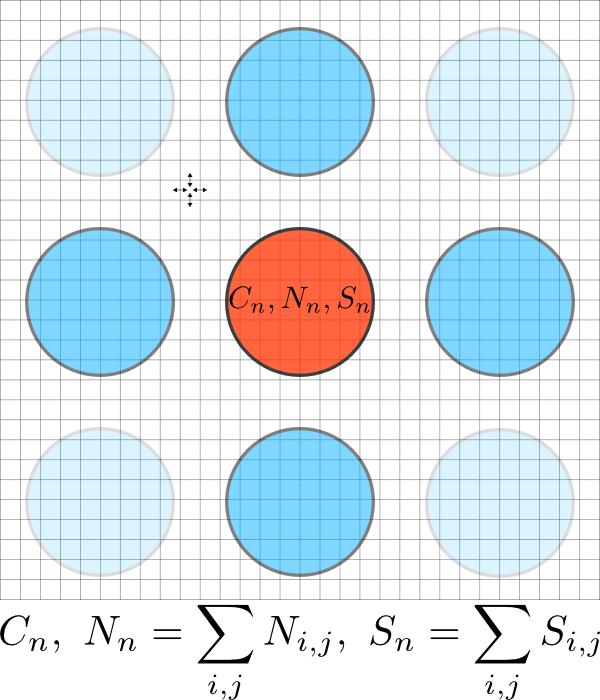
\includegraphics[width=\linewidth]{square_array_grid}
  \captionof{figure}{Schematic of a spatially-discretized
    two-dimensional model.}
  \label{fig:grid}
\end{Figure}

\begin{Figure}
  \centering
  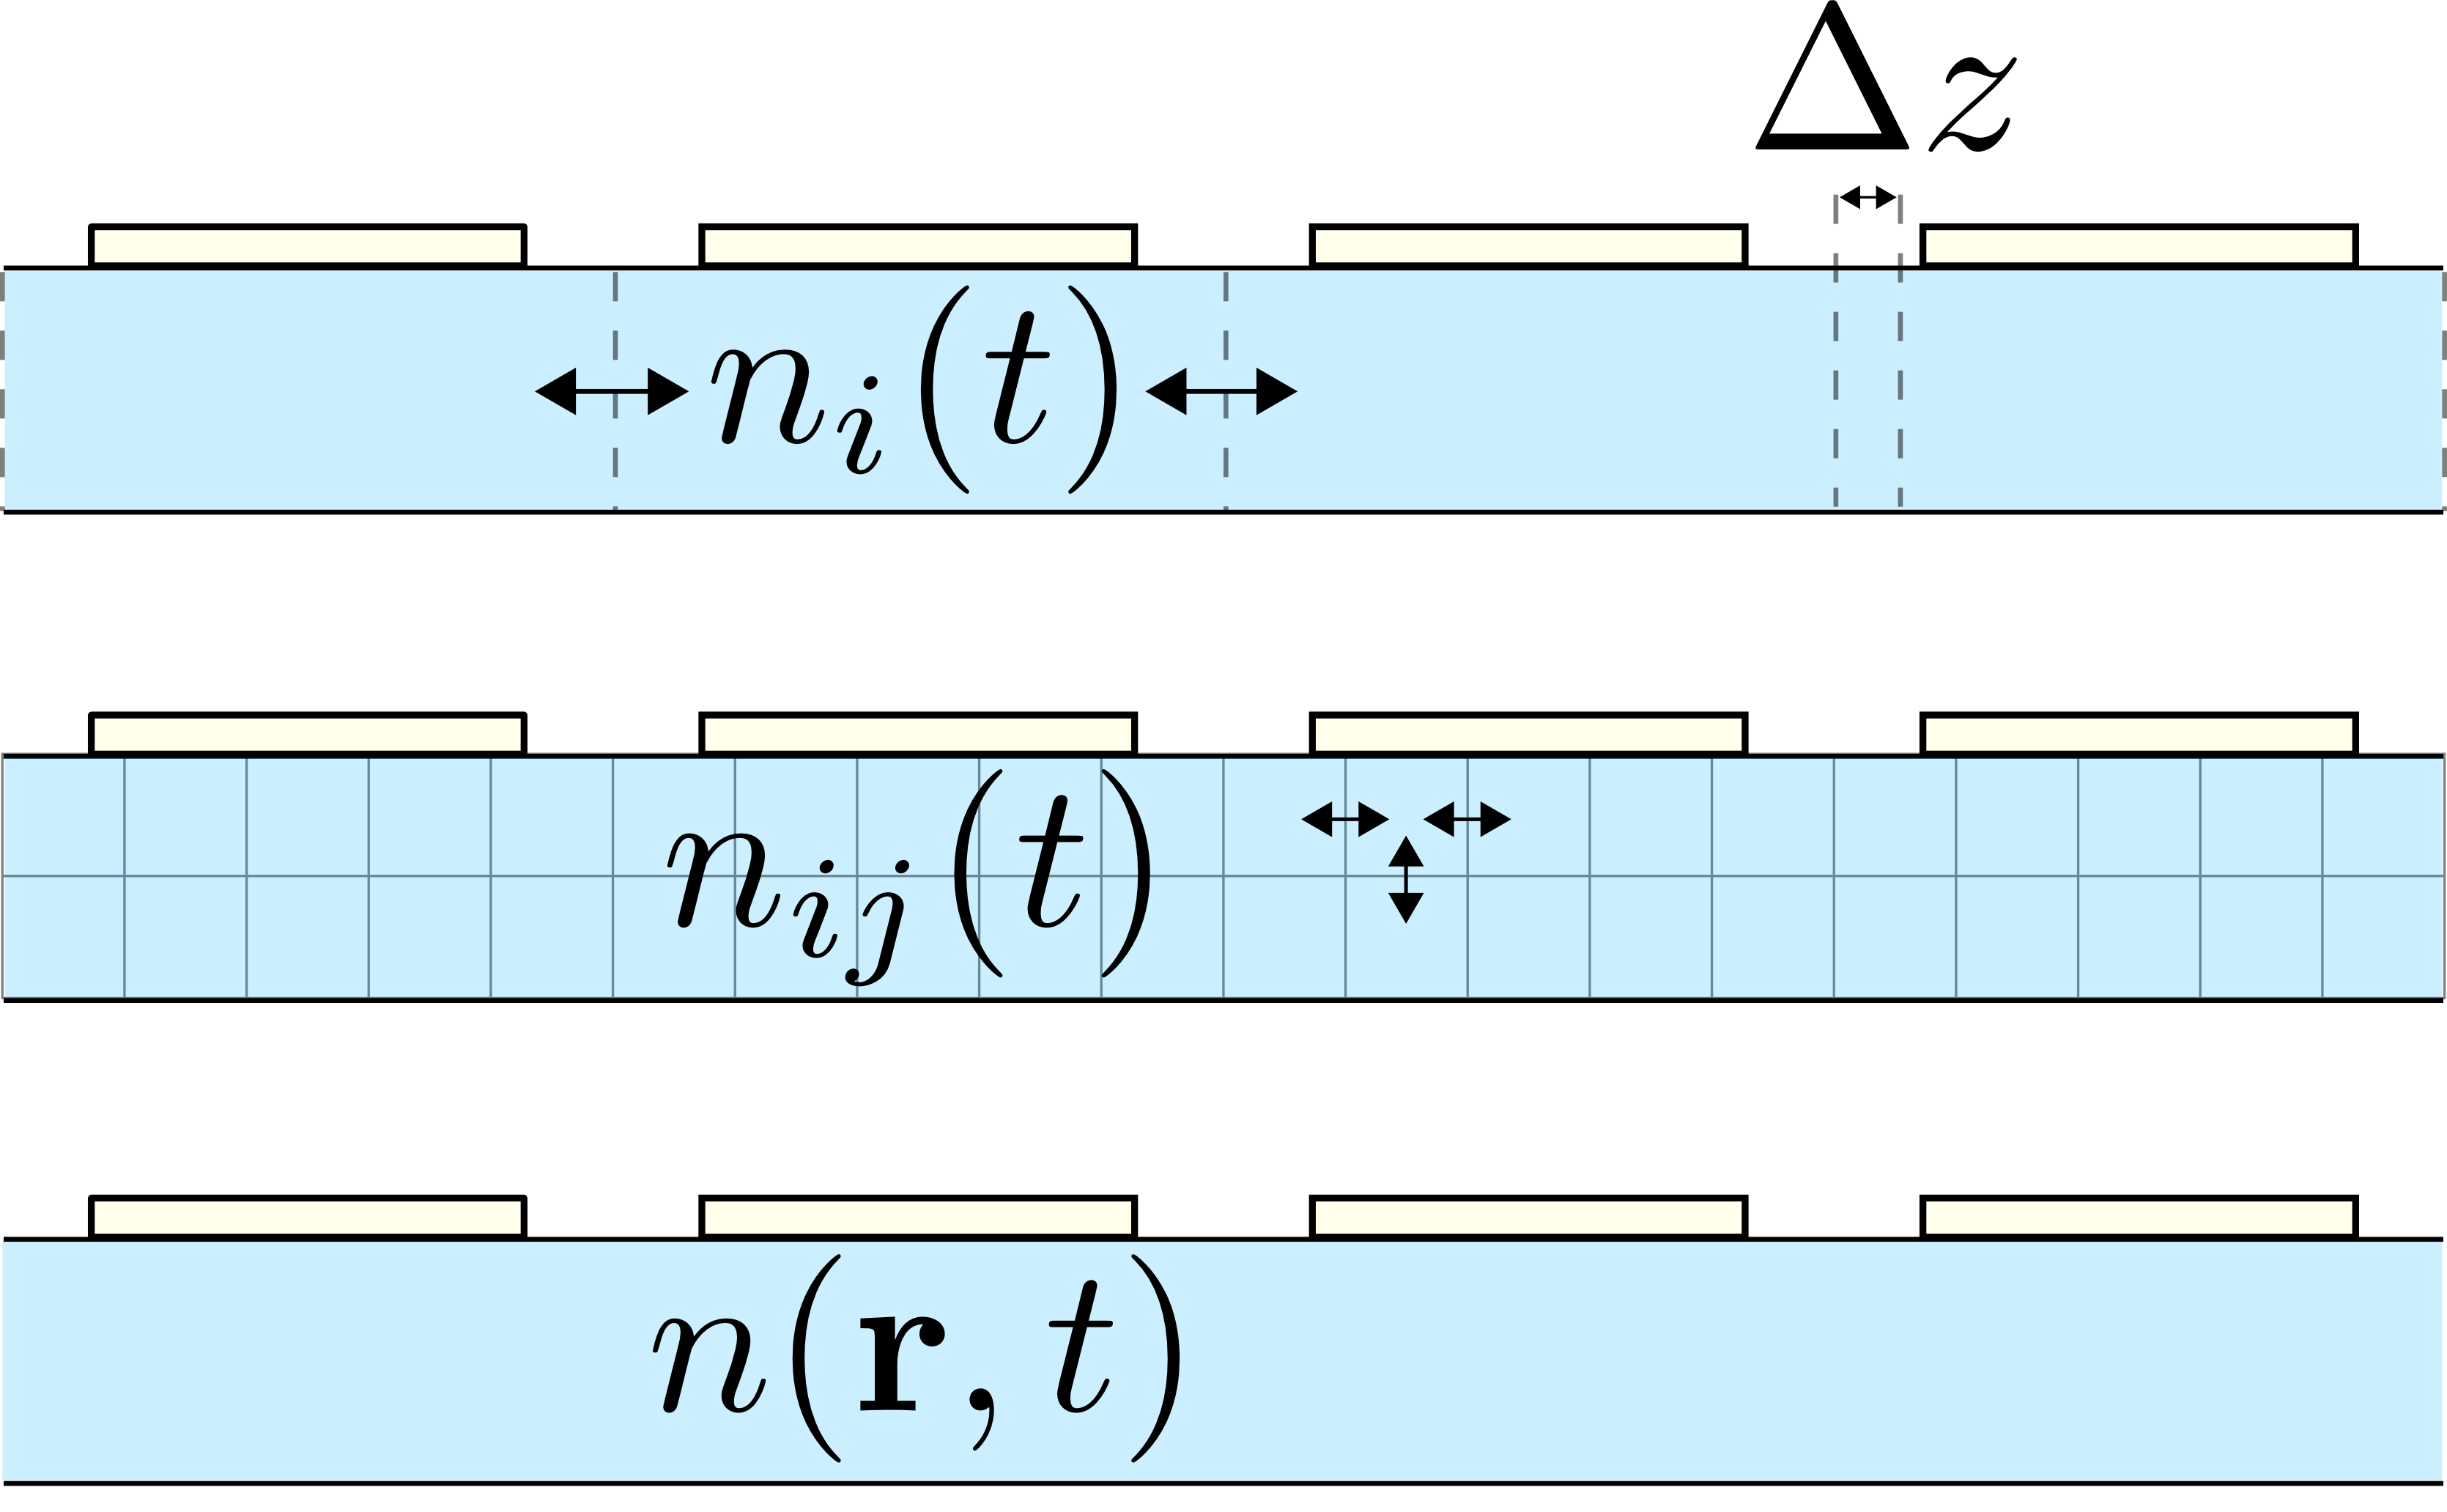
\includegraphics[width=\linewidth]{height_dep_miniqfa_delta_z}
  \captionof{figure}{Schematics of diffusion across agar height.}
  \label{fig:height_dependence}
\end{Figure}
% Could model movement of vertical or movement across it.

\subsection{Compare Experimental Designs}
\label{sec:comp-exper-designs}

If competition is present, without randomisation of culture location,
repeat observations may lead to overconfidence in fitness
estimates. As discussed in section~\ref{sec:initial_model}),
difficulties in measuring growth curves for cultures at the agar
boundaries would introduce a further systematic error. We will compare
growth parameters and fitness measures estimated from fits of the
competition and independence models for repeats with and without
randomisation and expect to find closer agreement between models when
randomisation is used. ?Or do we just do this using simulations? In
the case that the competition model is too slow to use in analysis of
large sets of data from high-throughput experiments, we still will be
able to determine how large a reduction in error can be achieved
through randomisation just using the independence model.

\begin{Figure}
  \centering
  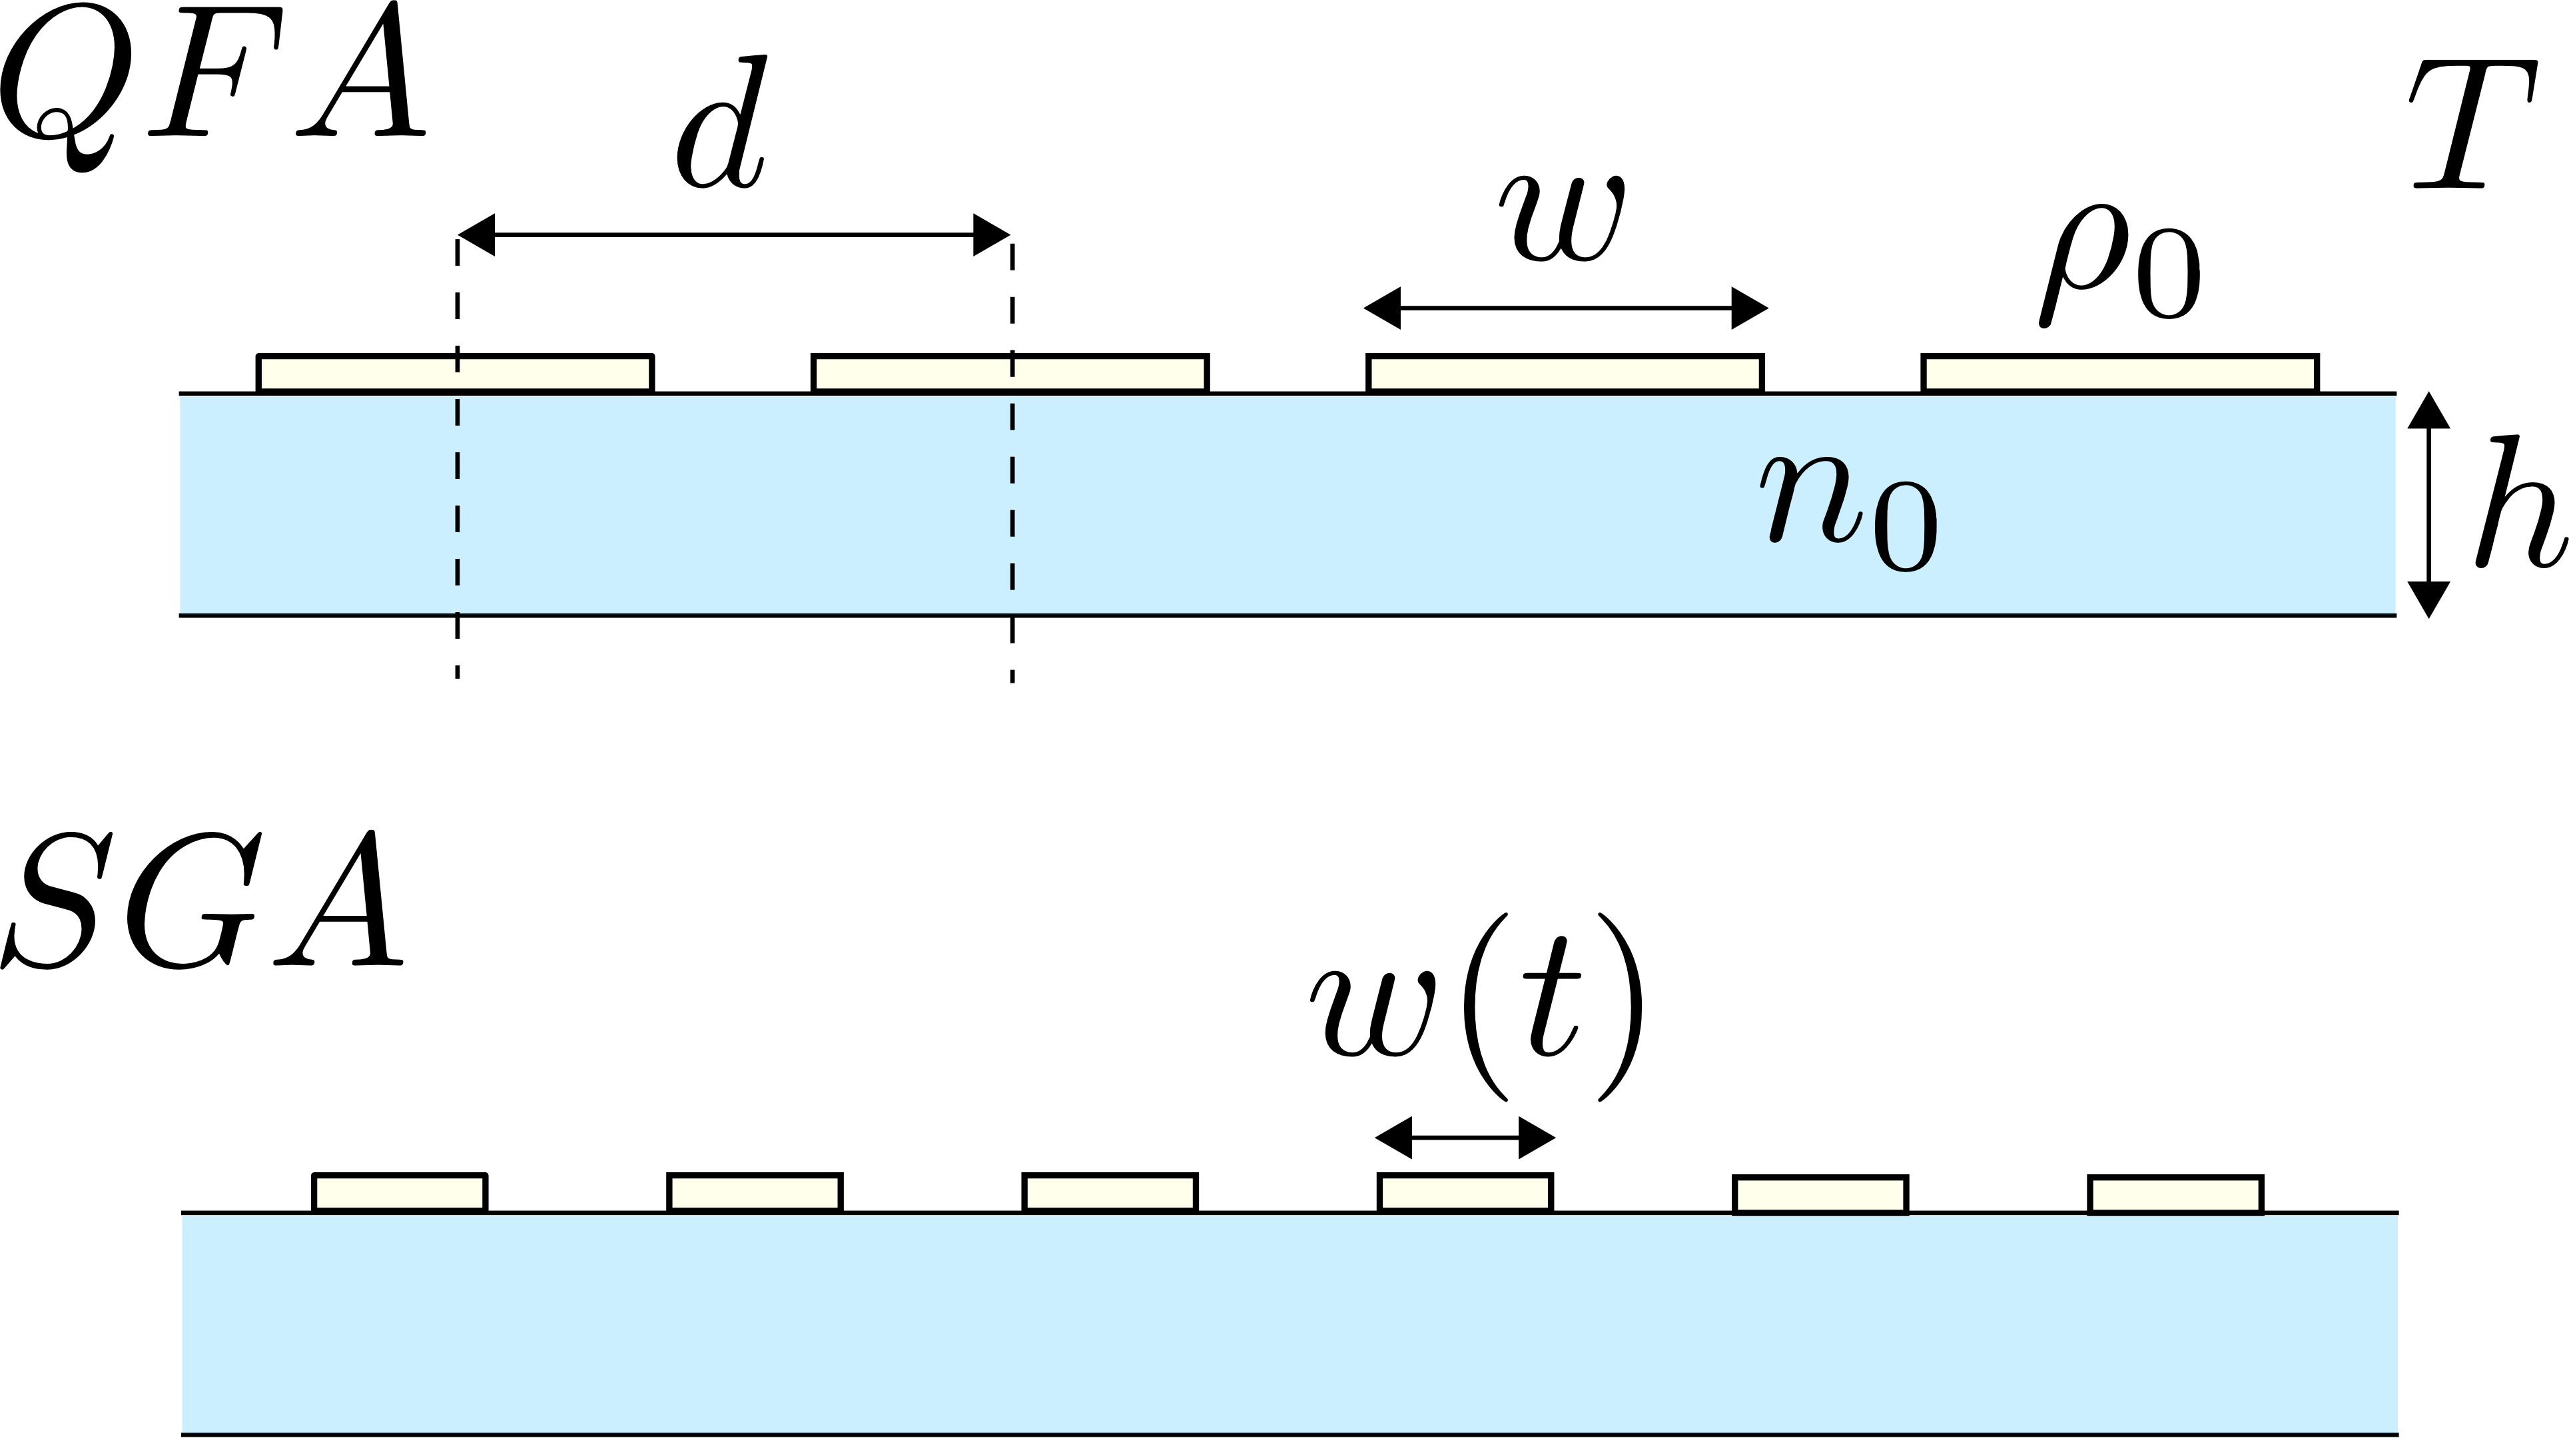
\includegraphics[width=\linewidth]{qfa_v_sga_vars}
  \captionof{figure}{QFA and SGA agars.}
  \label{fig:exp_vars}
\end{Figure}

If time allows, we wish to compare differences in CANS effects
between QFA and SGA designs. To do this we change the following variables:
\(\rho_{0}\), the initial concentration of cells, \(d\), the distance
between cultures, and \(w\), the diameter of cultures (see
Figure~\ref{fig:exp_vars}). For SGA, we also have to consider that the
diameter/area of cultures changes with time and account for this in
our models. In many SGA studies, culture area, rather than integrated
optical density (IOD), as in QFA, is used as a proxy for culture
density. \citet{Lawless2010} found that direct area measurements are
more noisy than IOD measurements and provide a worse fit to the
logistic model, introducing a bias to our data. Using
Colonyzer, we would instead take IOD measurements of SGA plates. We
should also account for the statistical advantage of SGA, in that
roughly five times more cultures that can be grown on SGA plates,
allowing for more repeats.

Simulations may be of use in comparing experimental variables, to study
the effect of one variable at a time. However, it is of greater
priority to compare SGA and QFA as they are currently performed,
because data and machinery already exists for these designs.

(?Pesumably already done somewhere? It is cheaper to use YEPD agars
than CSM agars, but these have a higher initial nutrient density
\(n_{0}\) and this reduces the time available to observe culture
growth. We could also choose to study this trade-off and see if there
is any reduction in CANS effects due to there being a shorter time for
diffusion to occur. ?However (A guess), we expect that CANS effects
would be small compared to the error from shorter observation time and
that a better approach would be to correct for CANS in CMS data either
directly or using randomisation.?)

\begin{Figure}
  \centering
  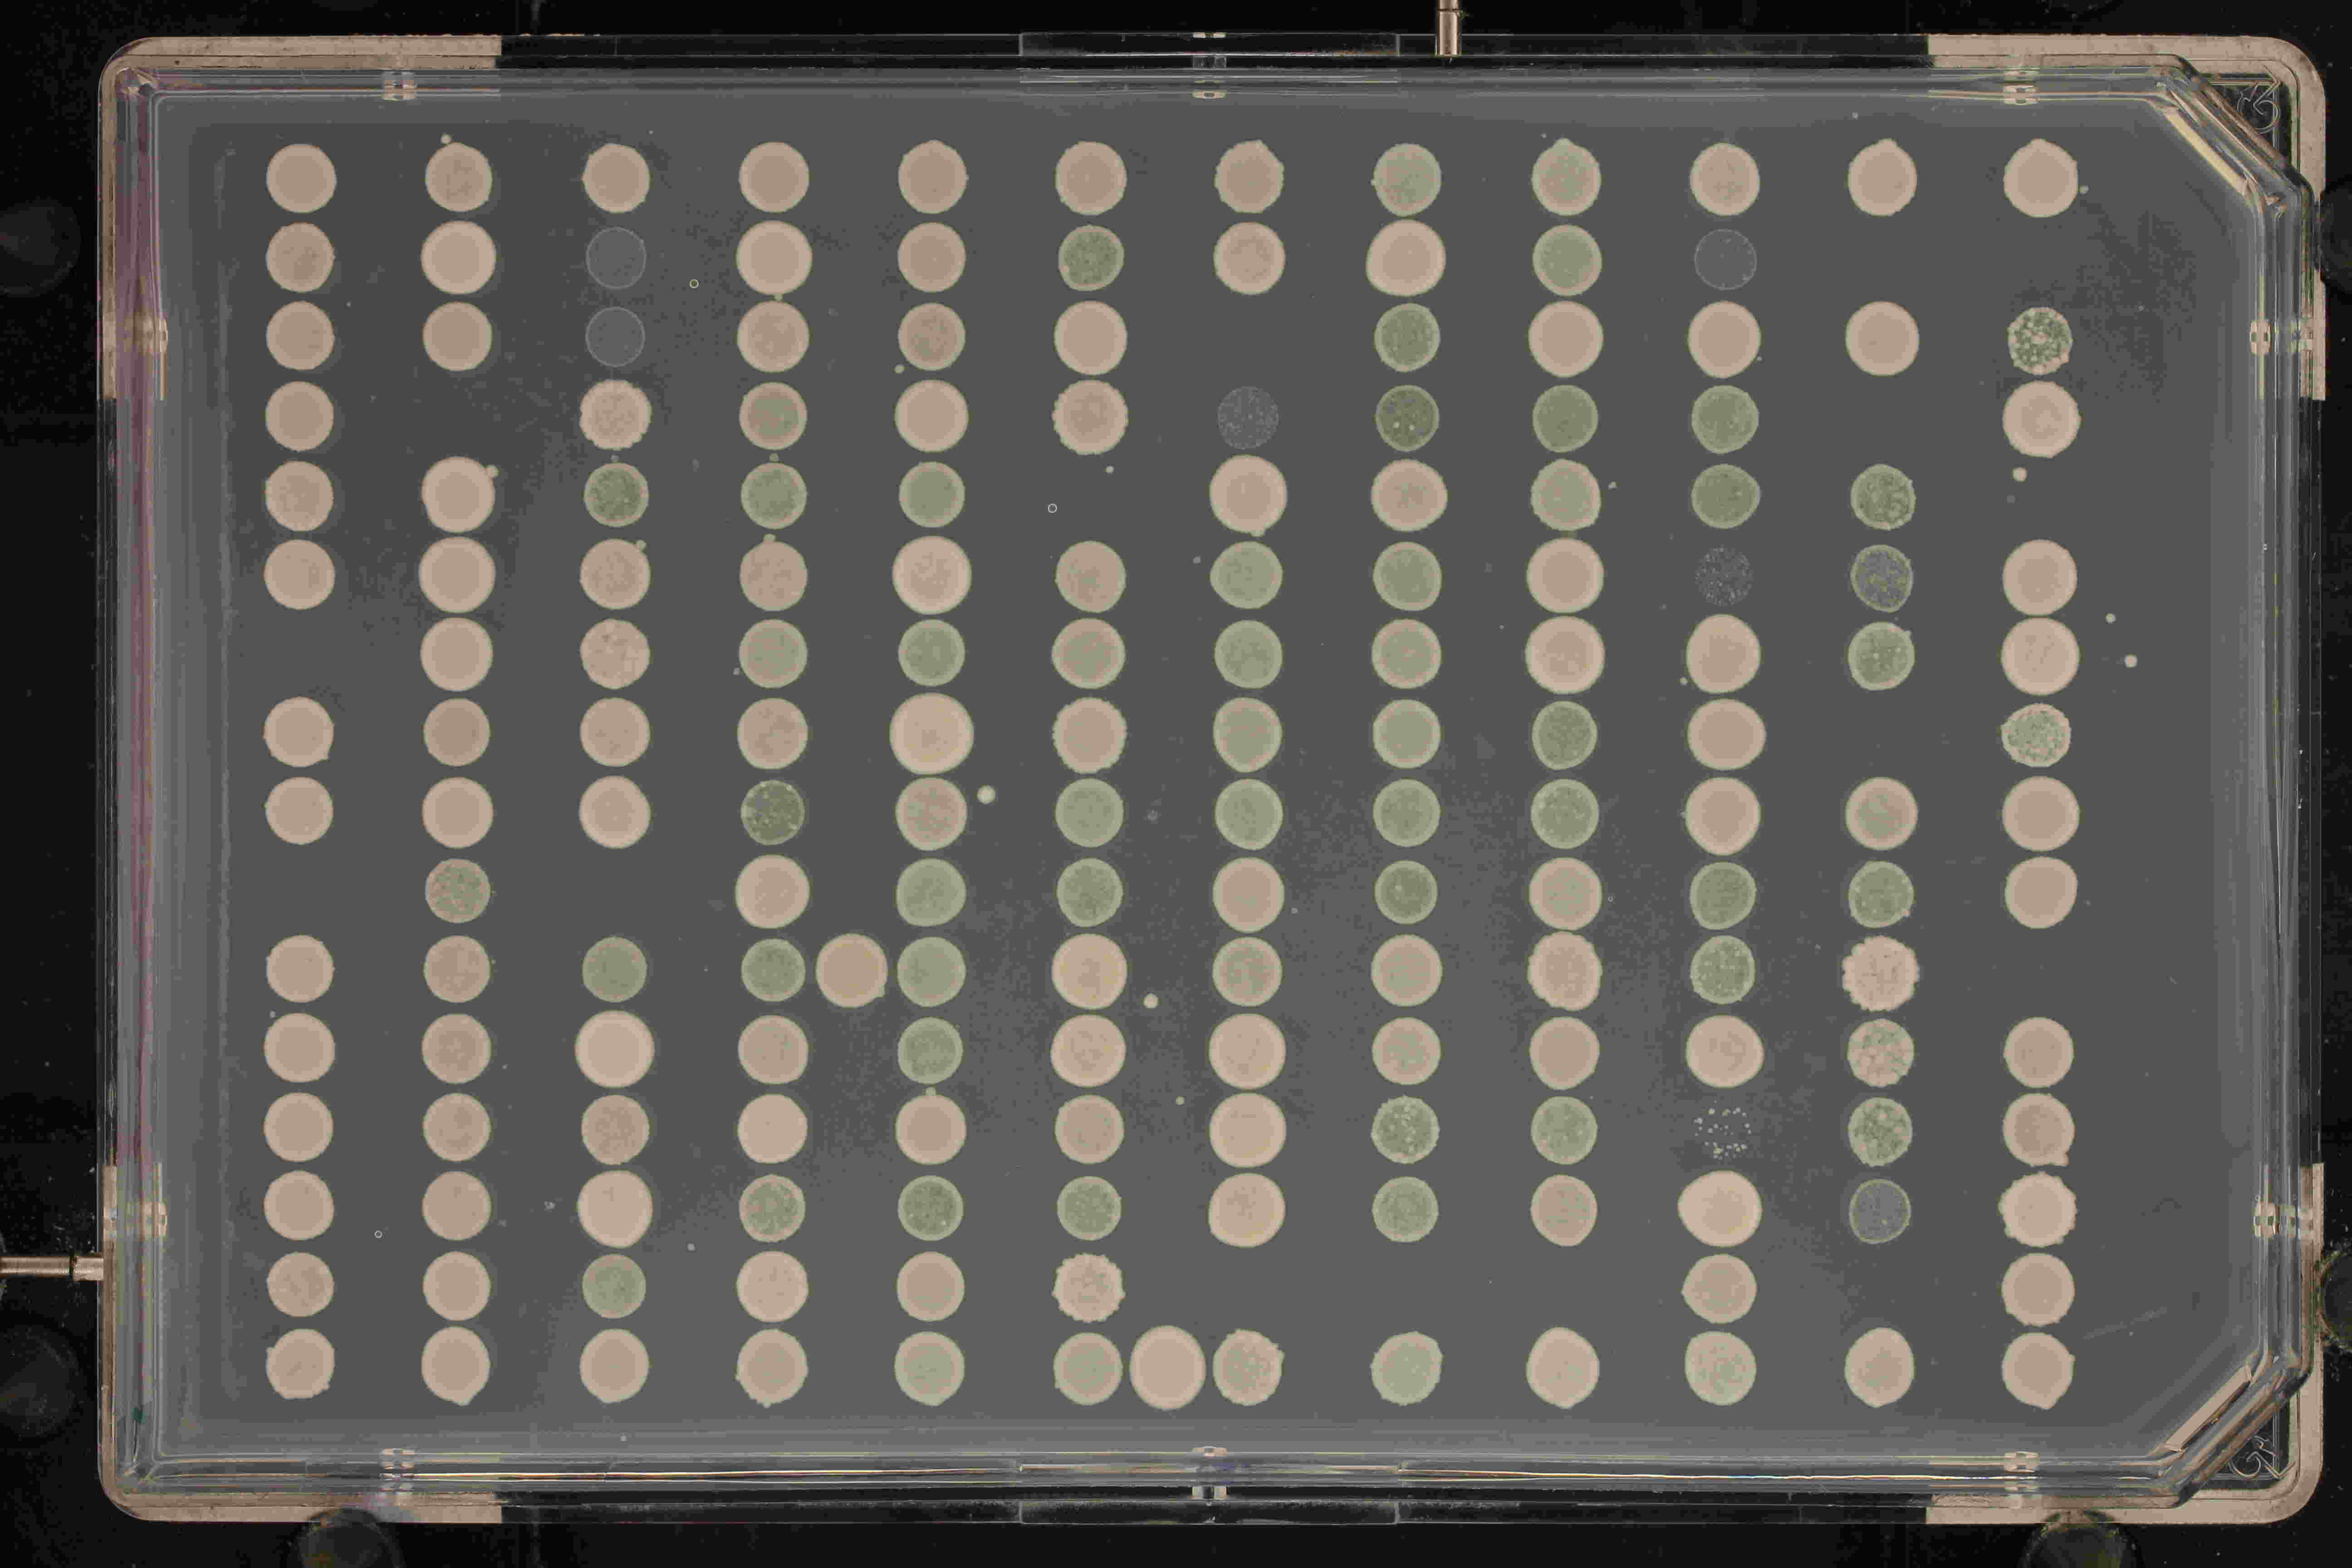
\includegraphics[width=\linewidth]{K000343_027_001_2015-02-21_19-38-08}
  \captionof{figure}{A miniQFA agar in which lines of locations
    (``stripes'') are left vacant. We can use a similar
    experimental setup, with uniform cultures in one dimension, to
    study diffusion at different agar heights in only two dimensions.}
  \label{fig:stripes}
\end{Figure}

\subsection{Package and Distribute}
\label{sec:package-distribute}
Already mentioned much of this in other parts of the
approach. Anything missing?

%%% Local Variables:
%%% mode: latex
%%% TeX-master: "proposal"
%%% End:
